\fancyfoot[C]{Kronberger}

%% Human-Computer Interaction System %%%%%%%%%%%%%%%%%%%%%%%

\chapter{Human-Computer Interaction System}

\section{Übersicht}
Das Human-Computer Interaction System ist, wie der Name schon verrät, die Komponente, welche als Schnittstelle zwischen dem Nutzer und dem gesamten elektrischen System dient. Durch es sollte die fehlerfreie Nutzung der Funktionen des Motorrades gewährleistet sein. Ebenso sollte es wichtige Fahrdaten und andere Informationen speichern und dem User anzeigen können.\\
Wichtig ist das System, troz der großen Komplexität, so intuitiv und nutzerfreundlich wie möglich zu gestallten.

\subsection{Grundfunktionen des Systems}
Die geplanten Funktionen des HCIS lassen sich grob in vier Grundfunktionen einteilen.
\begin{itemize}
	\item \textbf{Steuerung der Peripherie} \medskip\\
	Die Schalter und Buttons am Lenker, welche zuvor über den Kabelbaum die Leuchten, Blinker und die Hupe gesteuert haben. Werden nun über die General-purpose input/output (GPIO) anschlüsse des Raspberry Pi Micro Computers gesteuert.
	\item \textbf{Graphische Benutzeroberfläche}\medskip\\
Dient der Anzeige wichtiger Fahr- und Ladedaten, welche entweder in echtzeit oder über die Datenbankschnittstelle abgerufen und graphish angezeigt werden können.
	\item \textbf{Kommunikation mit den Steuereinheiten des Motorrades} \medskip\\
	Über CAN-Bus werden Daten von dem Batterie Management Systems (BMS) und der Curtis Motorsteuerung empfangen und an die Benutzeroberfläche zur echtzeit verwertung und an die Datenbankschnittstelle zur Langzeitsicherung der Fahrdaten weiter gegeben.
	\item \textbf{Speichern der relevanten Fahrdaten über die Datenbankschnittstelle} \medskip\\
Die über den CAN-Bus empfangenen Daten werden sofort an die Datenbankschnittstelle (Handler) weitergegeben um für Datenauswertung und Testberichte die Daten zu speichern. Ebenso bezieht das Diagnosesystem der Benutzeroberfläche die Daten über diese Schnittstelle.
\end{itemize}
\newpage


\subsection{Grundaufbau des Systems}
In der Abbildung \ref{fig:aufbauHCIS} wird der Grundaufbau des Systems und die Datenverbindungen der folgenden  Komponenten veranschaulicht.

\begin{itemize}
	\item Raspberry Pi - Die Steuereinheit des Systems.
	\\ Kommuniziert über CAN-Bus mit den anderen Steuerkomponenten des Motorrades.
	\item User Input - Die vorhandenen Schalter am Lenker des Motorrads werden über pull down Widerstände mit den Inputs des Raspberry Pis verbunden. 
	\item Peripherie - Die Grundkomponenten des Motorrades wie Scheinwerfer oder Hupe. Diese werden über Relais, welche an die Ausgänge des Raspberry pis angeschlossen sind, gesteuert.
	\item Dashboard - Der Bildschirm zur Anzeige der verarbeiteten Informationen. Dieser wird über HDMI und USB mit dem Raspberry Pi verbunden.
\end{itemize}

\begin{figure}[H]
	\begin{center}
		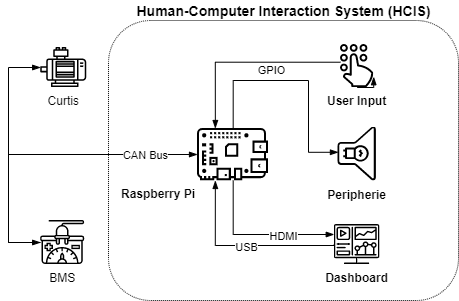
\includegraphics[scale=0.6]{figures/hcis/HCIS_Grundfunktion.png}
		\caption{Grundaufbau des Human-Computer Interaction Systems}
		\label{fig:aufbauHCIS}
	\end{center}
\end{figure}

Nicht in der Abbildung dargstellt ist die Versorgung der einzelnen Komponenten, welche in dem folgenden Abschnitt noch genauer erläutert wird.

\newpage

\subsection{Steuereinheit}
Als Basis zur Auswahl der Steuereinheit wurden die zuvor erläuterten Grundfunktionen herangeszogen genommen. Die Ausgewählte Steuereinheit sollte diese erfüllen können und ebenso Potential zur Erweiterung der Funktionen bieten. Genauso wichitg war das eine große Flexibilität und Individualität erreicht werden kann, um nicht in der Umsetzung unserer Ideen eingeschränkt zu sein. Zur Auswahl standen verschiedene Speicherprogrammierbare Steuerungen und Microcomputer, doch letzten endes überzeugte der Micrcomputer Raspberry Pi.

\begin{figure}[H]
	\begin{center}
		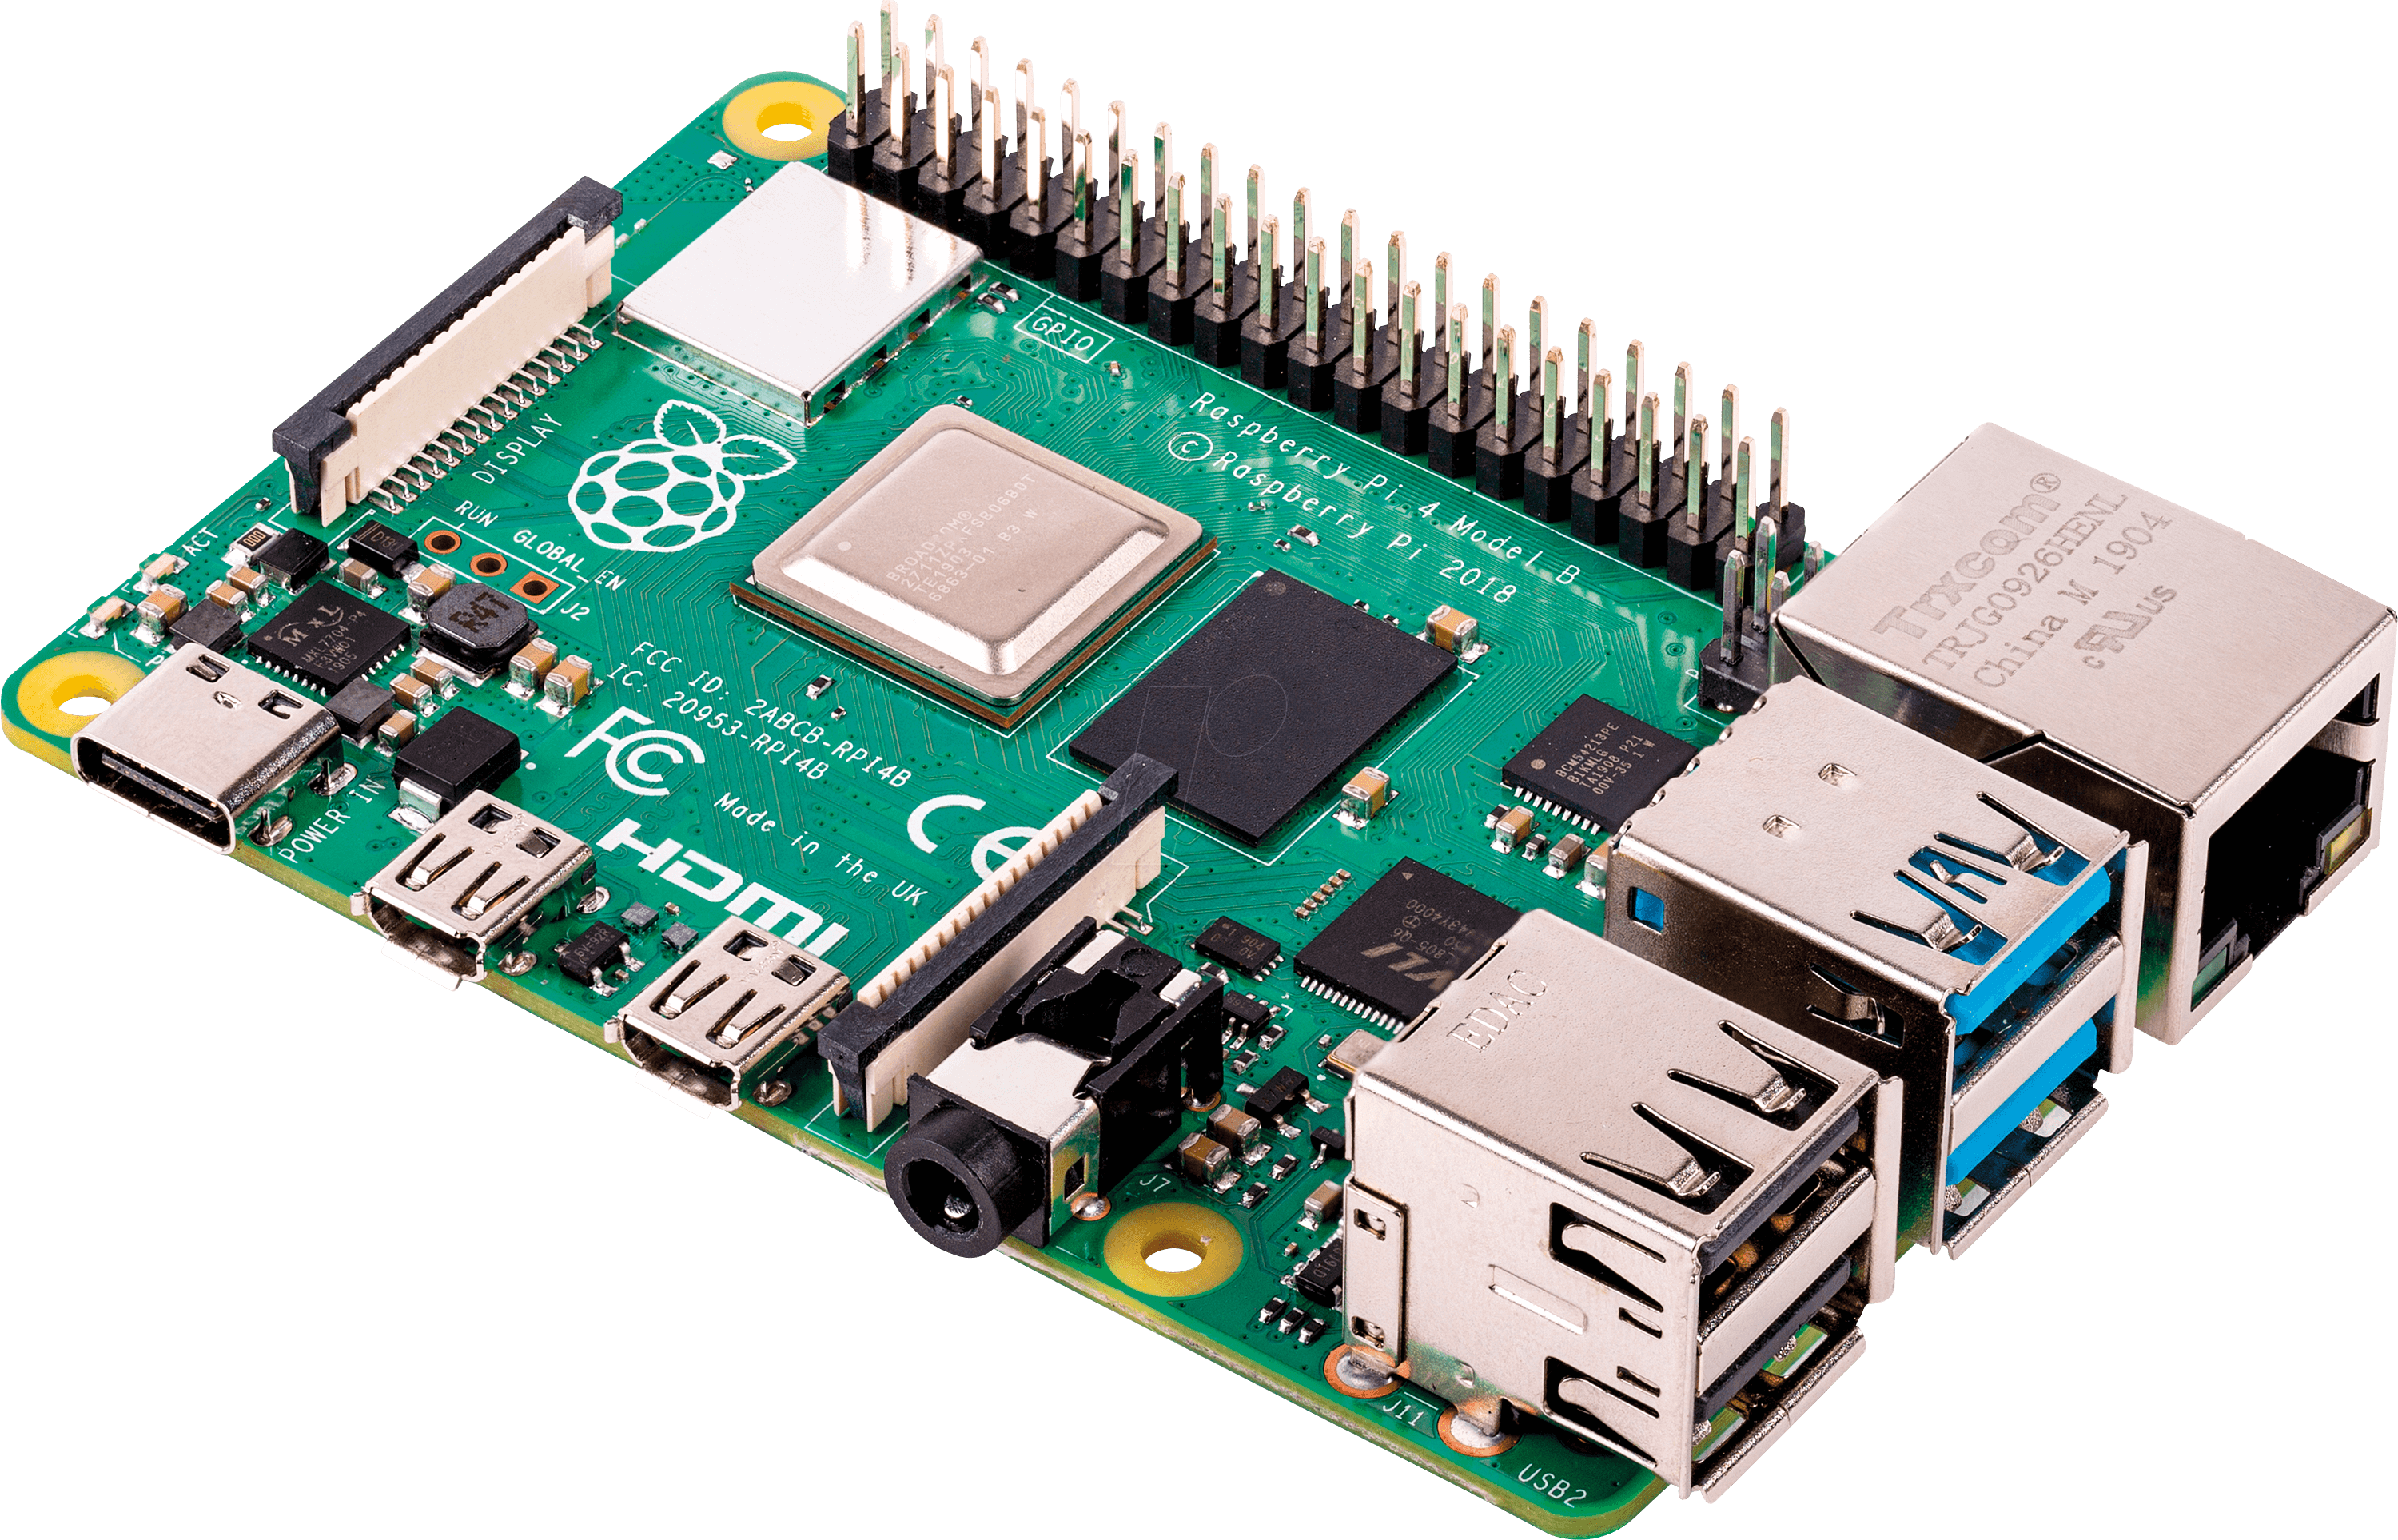
\includegraphics[scale=0.1]{figures/hcis/raspberryPi.png}
		\caption{Raspberry Pi - Steuereinheite des HCIS}
	\end{center}
\end{figure}

Durch 

\newpage


%% Versorgung %%%%%%%%%%%%%%%%%%%%%%%%%%%%%%%%%%%%%%%%%%%%%%% 

\section{Versorgung}

\subsection{Aufbau des Versorgungssystems}
Das Versorgungssysstem des Motorrades besteht aus zwei Spannungsebenen. Einer 12V Ebene zur Versorgung der Peripherie des Motorrades und einer 5V Ebene, welche nur den Raspberry Pi und seine Komponenten beinhaltet. Diese Ebenen werden durch DC-DC Wandler erzeugt, welche direkt an den 50,4V des Akkus des Motorrades angeschlossen werden. \\
Wichtig hierbei ist, dass alle ausgewählten Spannungswandler über einen Kurzschluss- und Überstrom-Schutz verfügen. Dies macht es uns möglich diese Versorgungssysteme, solange die Drähte auch nach dem maximalen Strom der Spannungswandler dimensioniert wurden, ohne jegliche Leitungs und Überstromschutzorgane aufzubauen. Denn die Spannungswandler schalten bei jeglichen Fehlern ab und verbrennen die Überschüssige Leistung über einen eingebauten Widerstand. Sobald der Fehler behoben wurde oder sich von selbst aufgelöst hat schalten sich die Spannungswandler automatisch wieder ein.
\subsubsection{12V Versorgungsysstem}
Um den Spannungswandler dimensionieren zu können mussten vorher alle Bauteile, welche über die 12V versorgt werden sollten, zusammengefasst werden, um die mindestens benötigte Wirkleistung des Spannungswandlers zu errechnen. 
\begin{table}[H]
\begin{center}
\begin{tabular}{|l|c|c|}
\hline
\textbf{Bauteilbezeichnung}     & \textbf{Spannung} & \textbf{Leistung} \\ \hline
Tagfahrlicht           & 12V      & 10W      \\ \hline
Abblendlicht           & 12V      & 10W      \\ \hline
Aufblendlicht          & 12V      & 20W      \\ \hline
Hupe                   & 12V      & 10W      \\ \hline
Rücklicht              & 12V      & 21W      \\ \hline
Kennzeichenbeleuchtung & 12V      & 5W       \\ \hline
Blinker links          & 12V      & 2 x 10W  \\ \hline
Blinker rechts         & 12V      & 2 x 10W  \\ \hline
Bildschirm             & 12V      & 12W      \\ \hline
\textbf{Gesamt}                 & \textbf{12V}      & \textbf{128W}     \\ \hline
\end{tabular}
\caption{Berechnung der Leistung des 12V-Systems}
\label{tab:leistung12V}
\end{center}
\end{table}

Der Spannungswandler wurde nun nach der größt möglichen Leistung, welche auftreten würde wenn alle Bauteile gleichzeitig auf höchstleistung betrieben werden, ausgelegt. Diese maximale Leistung beträgt, wie in der Tabelle \ref{tab:leistung12V} zu sehen, 128 Watt. Um noch Ausbaumöglichkeiten zu gewährleisten und uns nicht dem Leistungslimit des Wandlers zu nähern, haben wir uns für einen 300 Watt DC-DC Wandler von meanwell entschieden. 

\subsubsection{5V Versorgungssystem}

Die Leistung des Raspberry Pis ist mit einem Maximum von 6.2 Watt sehr klein und daher ist die Wahl des Spannungswandlers in diesem Fall nicht wirklich davon abhänging. Auch die Komponenten, welche angeschlossen werden, haben grunsätzlich keine erwähnenswerte Wirkleistung und müssen daher nicht genau einberechnet werden. Nun entschied nurmehr das Preis-Leistungs-Verhältnis sowie die Ausfallsicherheit des Spannungswandlers die Wahl.

\subsection{Abschalten der Spannungswandler}


\newpage

%% Steuerung der Peripherie %%%%%%%%%%%%%%%%%%%%%%%%%%%%%%%%%

\section{Steuerung der Peripherie}

Die Grundfunktionen wie Beleuchtung, Hupe und Blinker werden hier als Peripherie bezeichnet. Diese sollten so einfach wie möglich und vom Lenker aus zu bedienen sein. Ebenso müssen sie verlässlich gesteuert werden können. Daher haben wir uns entschieden diese Funktionen ebenso über den Raspberry Pi zu steuern, da dieser bei einem Fehler der Motorsteuerung über den eingebauten Puffer gespeist werden kann und daher diese wichtigen Funktionen bis zu einem sicheren Stillstand weiter betrieben und gesteuert werden können.\\
Dennoch ist in der Plan in Zukunft die Motorsteuerung, welche ebenso in der Lage wäre die Ausgänge abhängig von den Inputs zu schalten, diese Aufgabe übernehmen zu lassen, solange die Ausfallsicherheit ebenso gegeben wäre. Der Vorteil dieser Methode ist die Schaffung einer Zentralen Steuereinheit, welche alle Steueraufgaben in einem Bauteil vereinen kann.

\subsection{Hardware}

\subsubsection{Input}

Man kann einen GPIO Pin entweder als Eingang oder als Ausgang betreiben. Als Eingang kann er die Zustände High und Low einnehmen. Zum Beispiel von einem Schalter oder Taster. In der Regel beschaltet man die GPIOs des Raspberry Pis mit Widerständen, um Eingänge auf einen definierten Pegel zu setzten oder um den Strom zu begrenzen. Standartmäßig werden 10k Widerstände benutzt. Ob Pullup oder Pulldown ist grundsätzlich gleichgültig. Wir benutzen für das Einlesen der Eingänge 10k Pulldown Widerstände, um die Eingänge des Raspberry Pis nicht immer an einer Spannung angeschlossen zu haben.

\begin{figure}[H]
	\begin{center}
		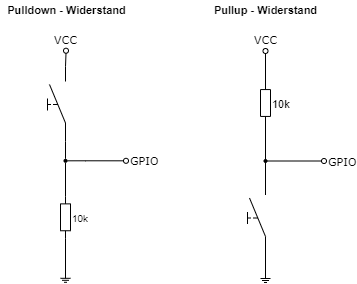
\includegraphics[scale=0.8]{figures/hcis/input.png}
			\caption{Anschlussplan Inputs}
			\label{fig:input}
	\end{center}
\end{figure}

\textbf{Pullup Widerstand}\\
Bei dem Nutzen eines Pullup Widerstands wird der GPIO Pin mit einem Widerstand auf die Spannnung von VCC gezogen. Der Grundzustand des Eingangs ist dann "High". Mit einem Schalter oder Taster wird der Eingang dann gegen Ground gezogen. Das heißt er hat solange der Schalter geschlossen ist den Zustand "Low".\\\medskip
\textbf{Pulldown Widerstand}\\
Bei dem Nutzen eines Pulldown Widerstands wird der GPIO Pin mit einem Widerstand auf die Spannnung von Ground gezogen. Der Grundzustand des Eingangs ist dann "Low". Mit einem Schalter oder Taster wird der Eingang dann gegen VCC gezogen. Das heißt er hat solange der Schalter geschlossen ist den Zustand "High".

\subsubsection{Output}

\begin{figure}[H]
	\begin{center}
		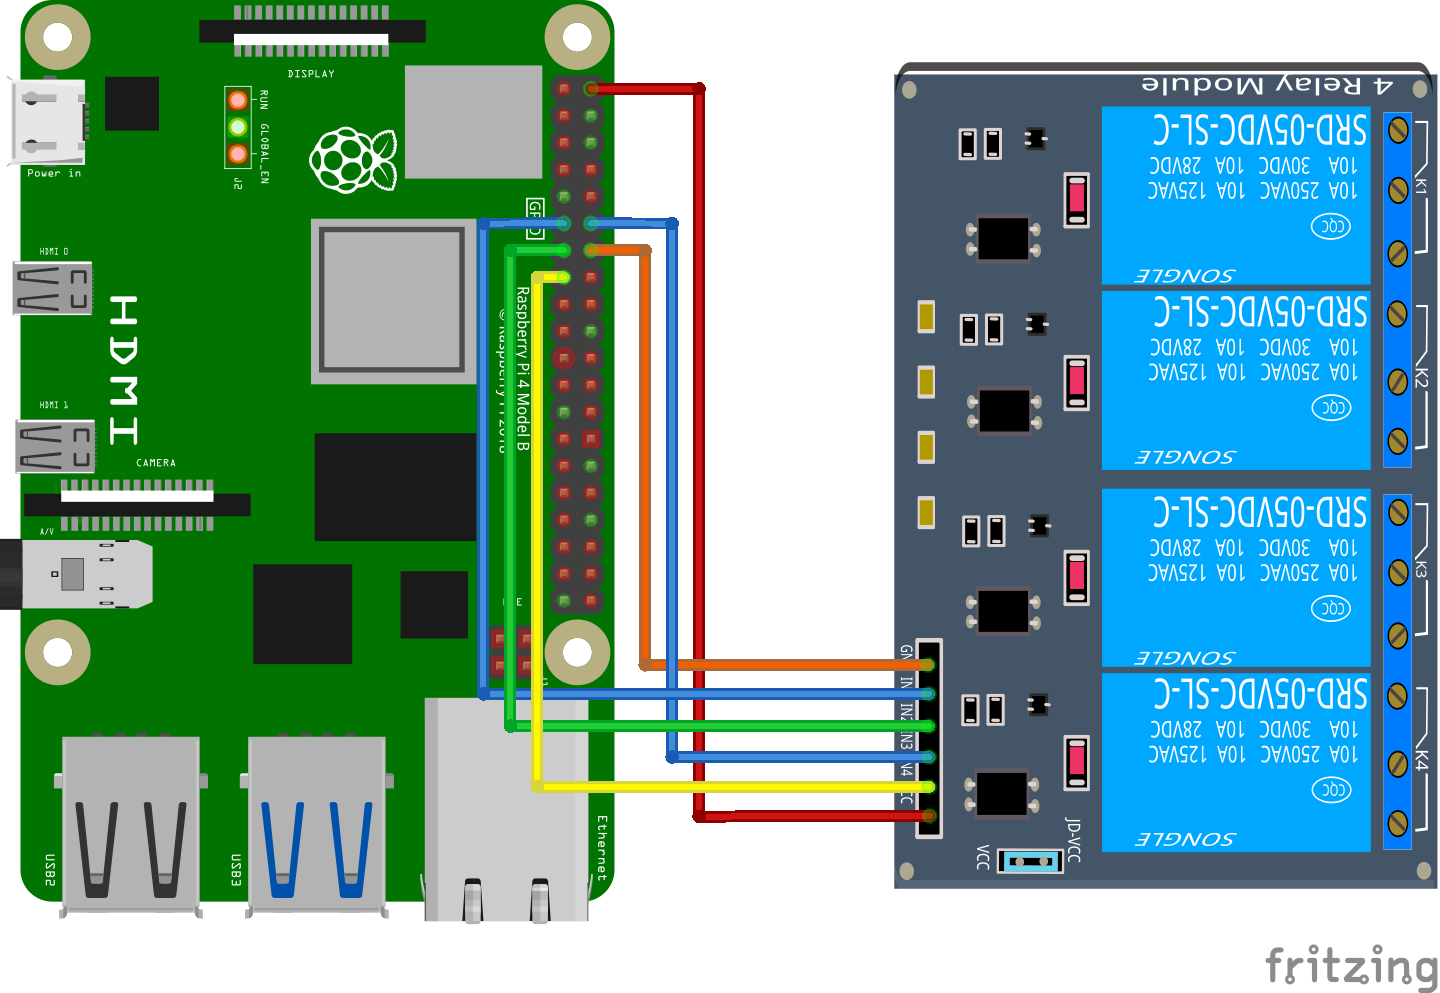
\includegraphics[scale=0.8]{figures/hcis/4ch_relai.png}
			\caption{Anschlussplan Relai}
			\label{fig:output}
	\end{center}
\end{figure}

\subsection{Software}

\subsubsection{GPIO Zero}

\subsubsection{Threading}

\newpage

%% Benutzeroberfläche %%%%%%%%%%%%%%%%%%%%%%%%%%%%%%%%%%%%%%%

\section{Benutzeroberfläche}
Die Benutzeroberfläche stellt die Verbindung zwischen dem Nutzer und dem Motorrad dar. Sie sollte während der Fahrt die Instrumententafel des Motorrades ersetzen und dem Nutzer die wichtigsten Fahrinformationen anzeigen. Sobald man zum Stillstand gekommen ist, wird es möglich Einstellungen zu ändern und die aufgezeichnetetn Fahrdaten anzeigen zu lassen. Ebenso kann der Akkuladestatus und Informationen über Fehler im System entnommen werden.

\subsection{Hardware}

Zur Anzeige und Bedienung wird ein 11.6 Zoll Kapazitives Touch LCD Display verwendet. Es besitzt eine FullHD Auflösung (1920x1080), was für eine professionelle Darstellung essenttiell ist. Ebenso hat es ein schützendes ABS Gehäuse, welches troz fehlender IPX zertivizierung das Abdichten ermöglicht. Die Versorgungsspannung beträgt 12V, was ident zu den anderen Komponenten am Motorrad ist und daher die Versorgung sehr vereinfacht, es kann also über den gleichen Spannungswandler versorgt werden.

\begin{figure}[H]
	\begin{center}
		\includegraphics[scale=0.45]{figures/hcis/display_maße.png}
		\caption{Touch Panel Maße}
		\label{fig:panel}
	\end{center}
\end{figure}

Die Auflösung und die Größe des Touch Panels wirkt sich stark auf das Design der Benutzeroberfläche aus. Es muss die Größe der Icons und der anderen Designelemente so angepasst werden, dass sie einerseits gut ersichtlich und andererseits einfach über Touch zu bedienen sind.\\
Touchdisplay

\newpage

\subsubsection{Befestigung}
Das Touchpanel besitzt M4 verschraubungen in einem Abstand von 75mm x 75mm und kann daher einfach an Wänden oder Platten verschraubt werden. Um Den Bildshirm nun in einer ähnlichen Position wie die Intrumententafel zu befestigen wird eine 100mm x 210mm x 1.5mm Aluminum Platte - wie in der Abbildung zu sehen - gebogen und mit Löchern versehen. Um diese Halterung nun an dem Motorrad zu befestigten werden die Verschraubungen der alten Instrumententafel verwendet.

\begin{figure}[H]
	\begin{center}
		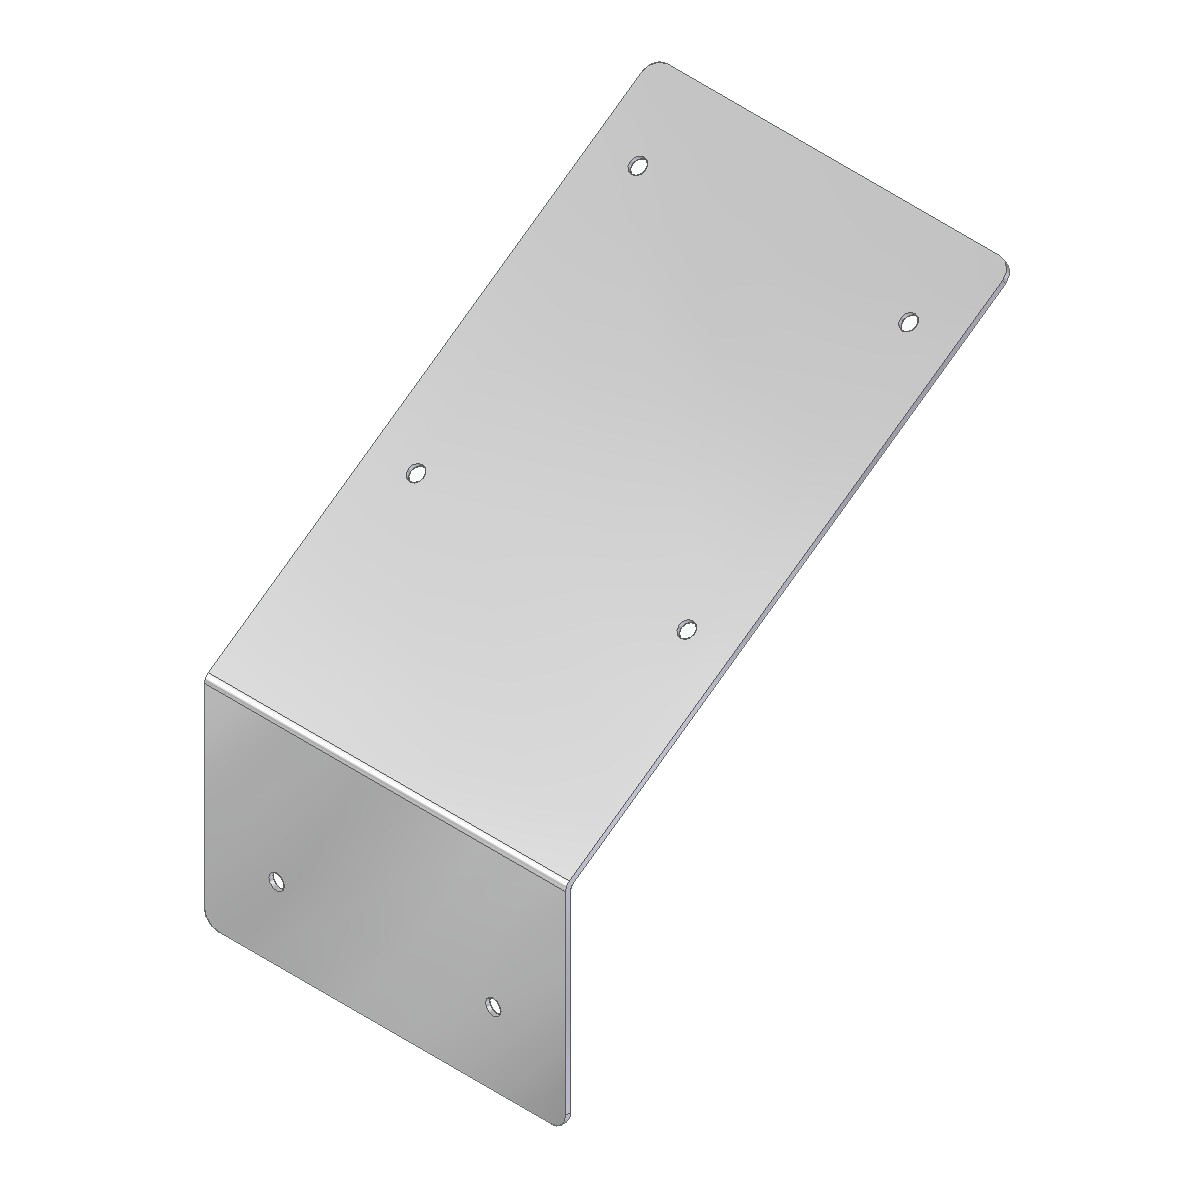
\includegraphics[scale=0.18]{figures/hcis/befestigung_display.png}
		\caption{Befestigung des Displays}
		\label{fig:befestigung}
	\end{center}
\end{figure}

\subsection{Software}
Bevor die Software für die Benutzeroberfläche verfasst wurde, musste das Design, Funktionen sowie die angezeigten Informationen geplant werden, um einen reibungslosen Workflow beim Entwickeln des front ends zu gewährleisten. Design Elemente wurden zuvor in Adobe Illustrator vorgefertigt. In den folgenden Seiten wird das Ergebnis dieses Prozesses erläutert.
\subsubsection{Aufbau}
Die nachfolgende Abbildung zeigt den grundsätzlichen Programmaufbau der Benutzeroberfläche. Die einzelnen Fenster werden als Tabelle mit ihren angezeigten Informationen dargestellt. Dies is wichtig da jede dieser Informationen vom back end an das front end gesendet werden müssen.\\
Ebenso sind in den letzten Zeilen der Tabellen die QML-Elemente zur Navigation zwischen den einzelnen Fenstern niedergeschrieben. Diese müssen auch schon in der frühen phase der Entwicklung der Benutzeroberfläche definiert werden.

\begin{figure}[H]
	\begin{center}
		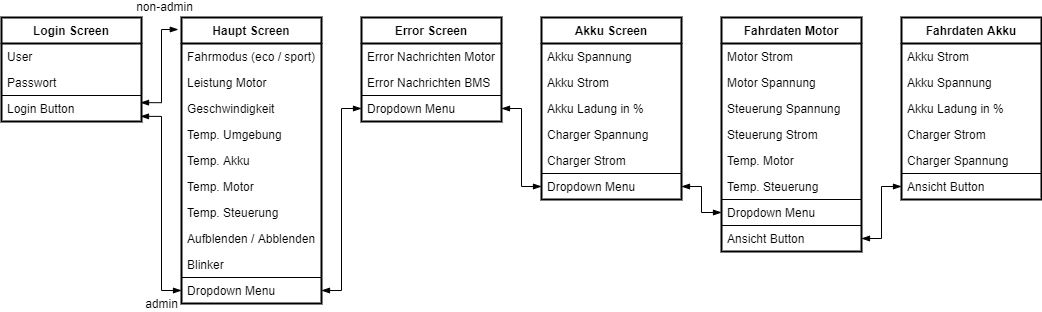
\includegraphics[scale=0.4]{figures/hcis/gui_aufbau.png}
		\caption{Aufbau der Graphischen Benutzeroberfläche}
		\label{fig:aufbauGUI}
	\end{center}
\end{figure}

\newpage

\subsubsection{Nutzer / Berechtigungen}

\subsection{Komponenten}

Komponenten sind wiederverwendbare, gekapselte QML-Elemente mit genau definierten Schnittstellen. Komponenten werden häufig durch Komponentendateien definiert, das heißt durch QML-Dateien. Wichtig ist dabei die Definierung von Schnittstellen sowie Properties und Signals (Siehe \ref{sec:slots}).\\\medskip
\begin{large}
\textbf{Properties}\\\medskip
\end{large}

Der Property eines Objektes kann ein statischer Wert zugewiesen werden, der konstant bleibt, bis ihm explizit ein neuer Wert zugewiesen wird. Um QML und seine integrierte Unterstützung für dynamisches Objektverhalten optimal zu nutzen, verwenden die meisten QML-Objekte jedoch Propertysbindings.\\
Propertysbindings sind eine Kernfunktion von QML, mit der Beziehungen zwischen verschiedenen Objekteigenschaften festgelegt werden können. Wenn sich die Abhängigkeiten einer Property im Wert ändern, wird die Eigenschaft automatisch gemäß der angegebenen Beziehung aktualisiert.\\
Hinter den Kulissen überwacht die QML-Engine die Abhängigkeiten der Eigenschaft. Wenn eine Änderung erkannt wird, wertet die QML-Engine den Bindungsausdruck erneut aus und wendet das neue Ergebnis auf die Eigenschaft an.

\subsubsection{Navigations Menu}

Das Navigations Menu ist ein dropdown menu, welches zur Navigation zwischen den verschiedenen Pages benützt wird. Sobald man sich eingelogt hat wird das Menu angezeigt und kann ausgewählt werden. Das Menu wird abhänigig von den Berechtiungen des Benutzers angepasst.

\begin{figure}[H]
	\begin{center}
		
\includegraphics[scale=0.2]{figures/hcis/component_menu.png}
		\caption{GUI Komponente - Navigation Menu}
		\label{fig:kompNavigation}
	\end{center}
\end{figure}

Die funtion welche

\subsubsection{Balken Anzeige}

\begin{figure}[H]
	\begin{center}
		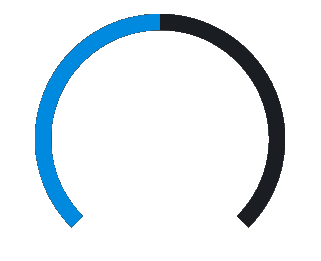
\includegraphics[scale=0.5]{figures/hcis/component_bar.png}
		\caption{GUI Komponente - Balken Anzeige}
				\label{fig:kompBalken}
	\end{center}
\end{figure}

\subsubsection{Graph}

\newpage

\subsection{Program Fenster}

\subsubsection{Login}

\begin{figure}[H]
	\begin{center}
		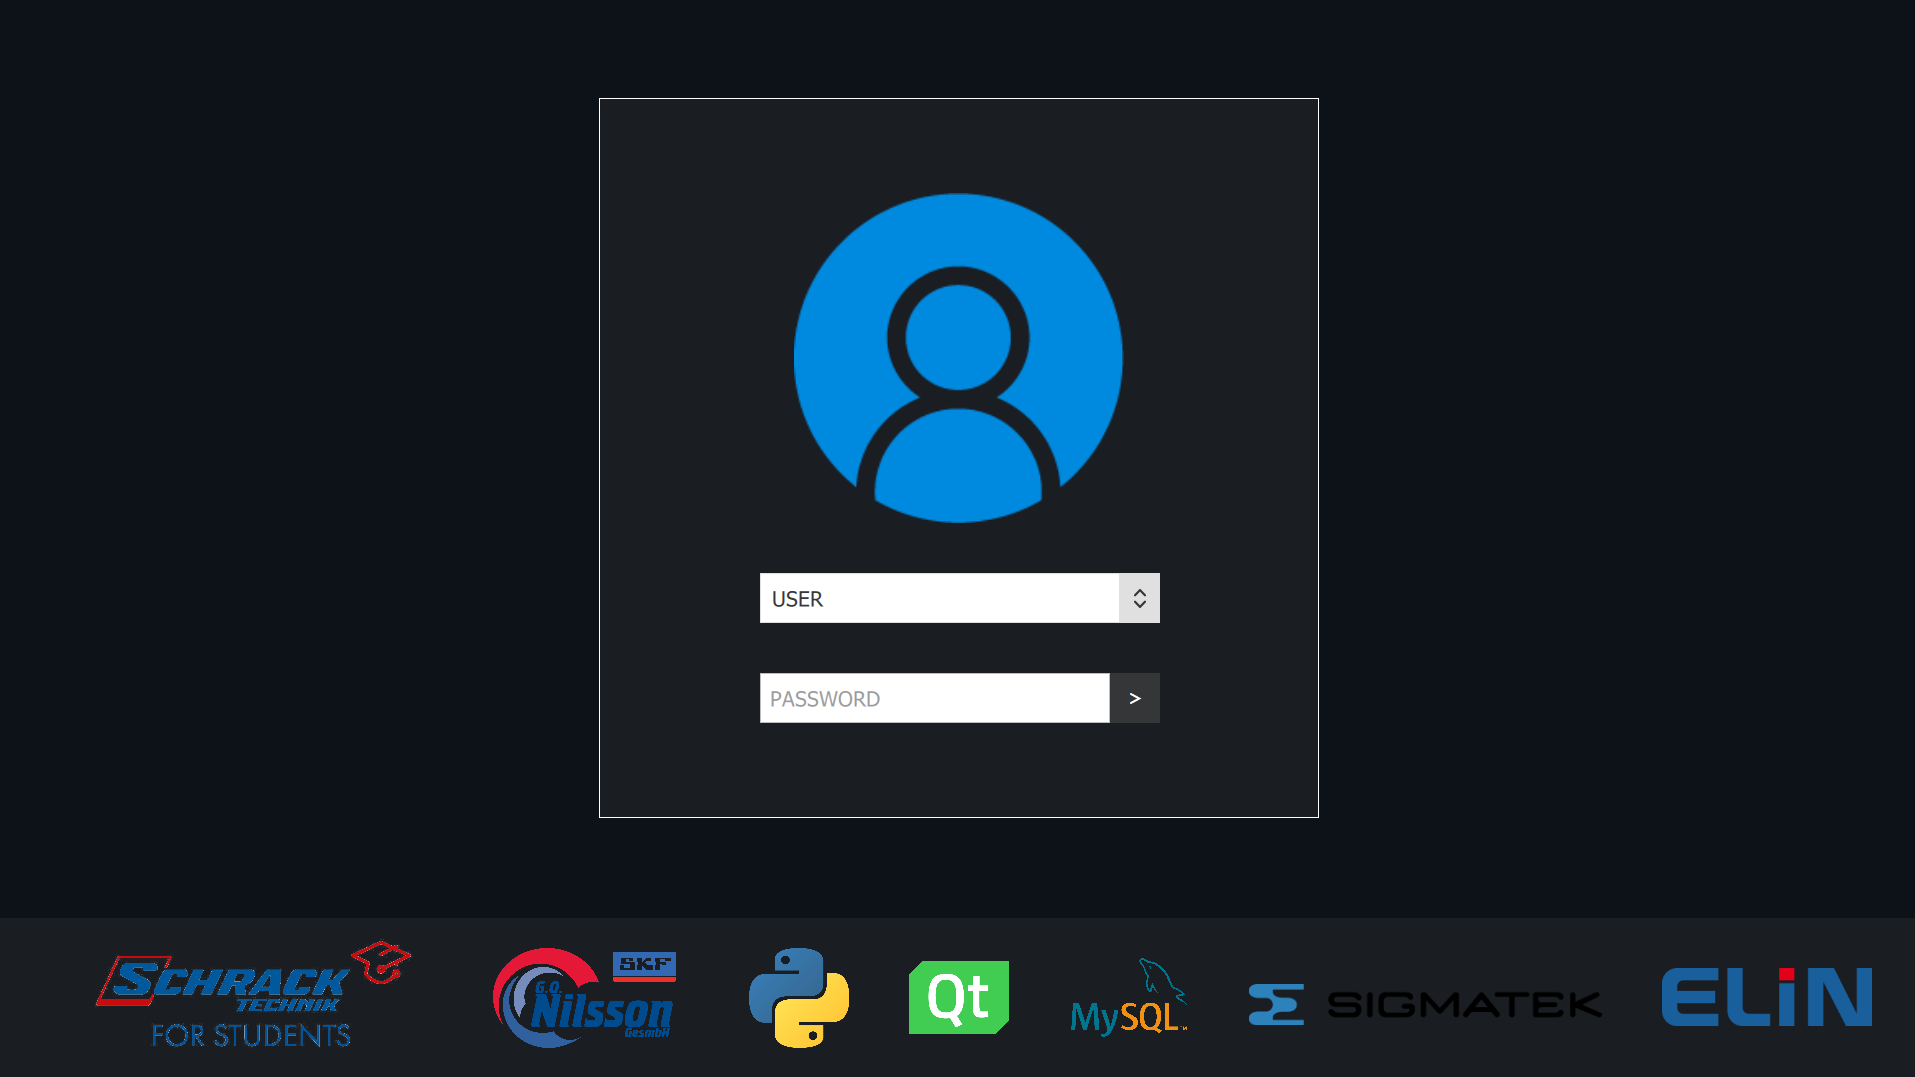
\includegraphics[scale=0.24]{figures/hcis/window_login.png}
			\caption{GUI Fenster - Login Menu}
			\label{fig:pageMenu}
	\end{center}
\end{figure}

\subsubsection{Fahrdaten}

\begin{figure}[H]
	\begin{center}
		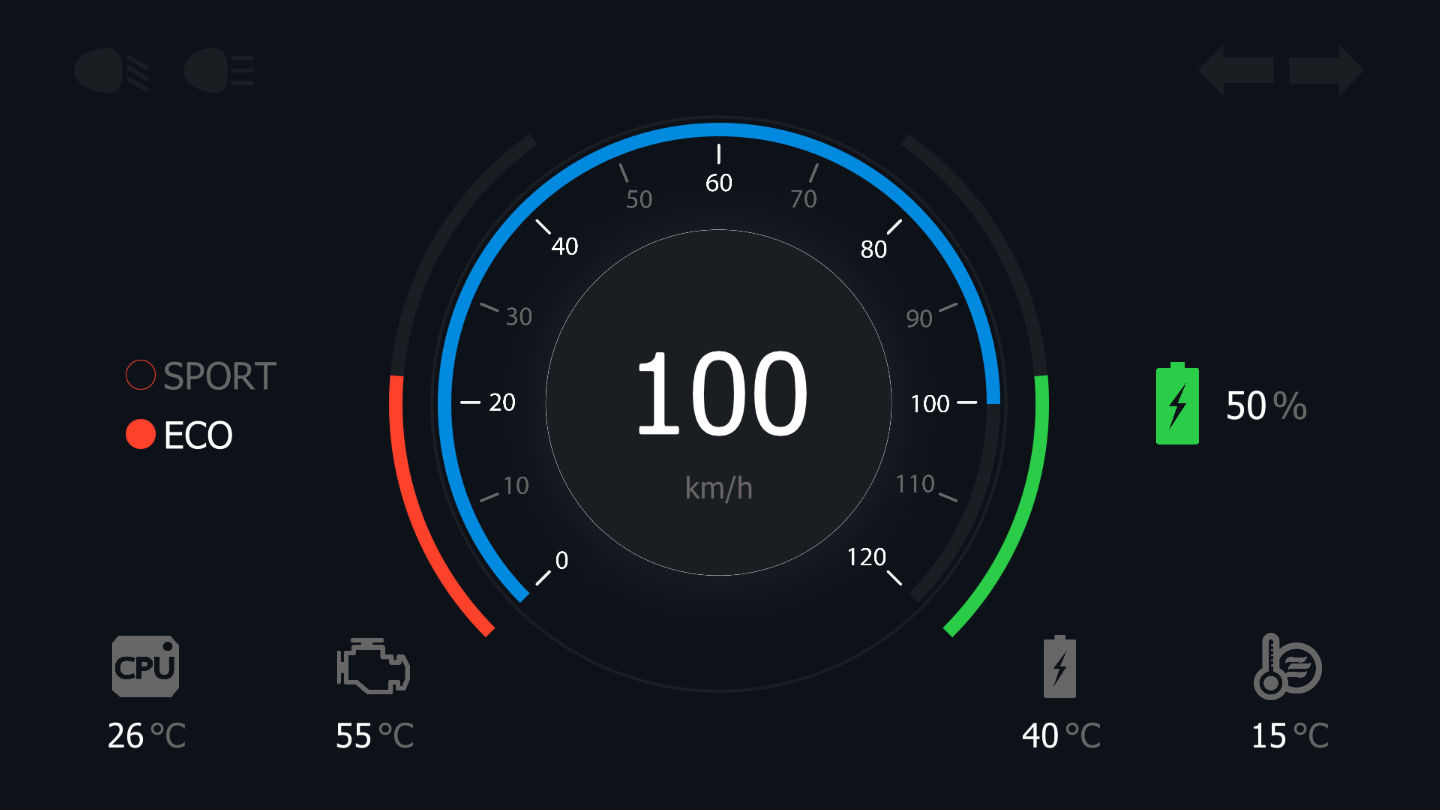
\includegraphics[scale=0.24]{figures/hcis/window_dashboard.png}
			\caption{GUI Fenster - Fahrdaten}
			\label{fig:pageDash}
	\end{center}
\end{figure}

\newpage

\subsubsection{Akku- und Ladedaten}

\begin{figure}[H]
	\begin{center}
		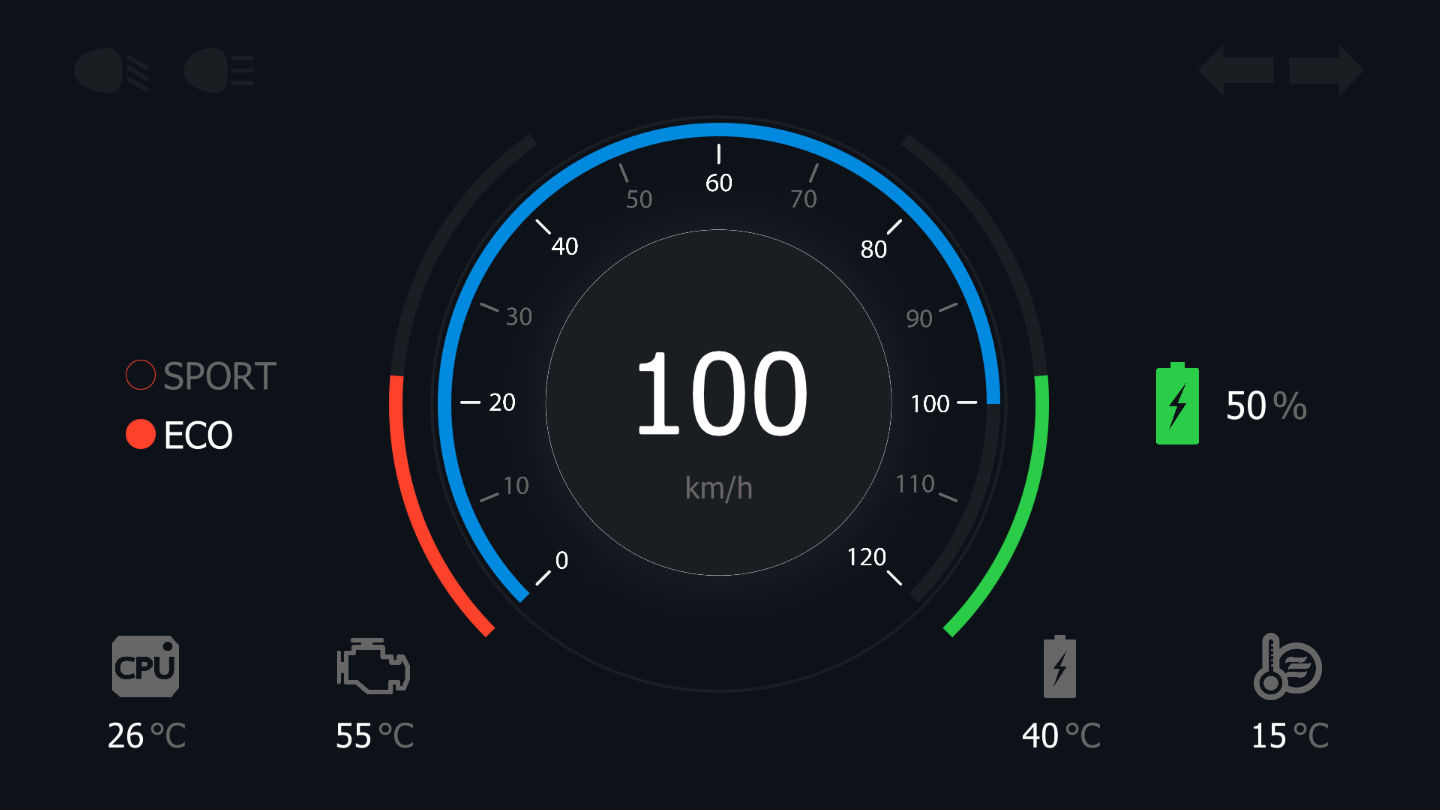
\includegraphics[scale=0.24]{figures/hcis/window_dashboard.png}
			\caption{GUI Fenster - Akkudaten}
			\label{fig:pageAkku}
	\end{center}
\end{figure}

\subsubsection{Fahrdaten Diagnose}

\begin{figure}[H]
	\begin{center}
		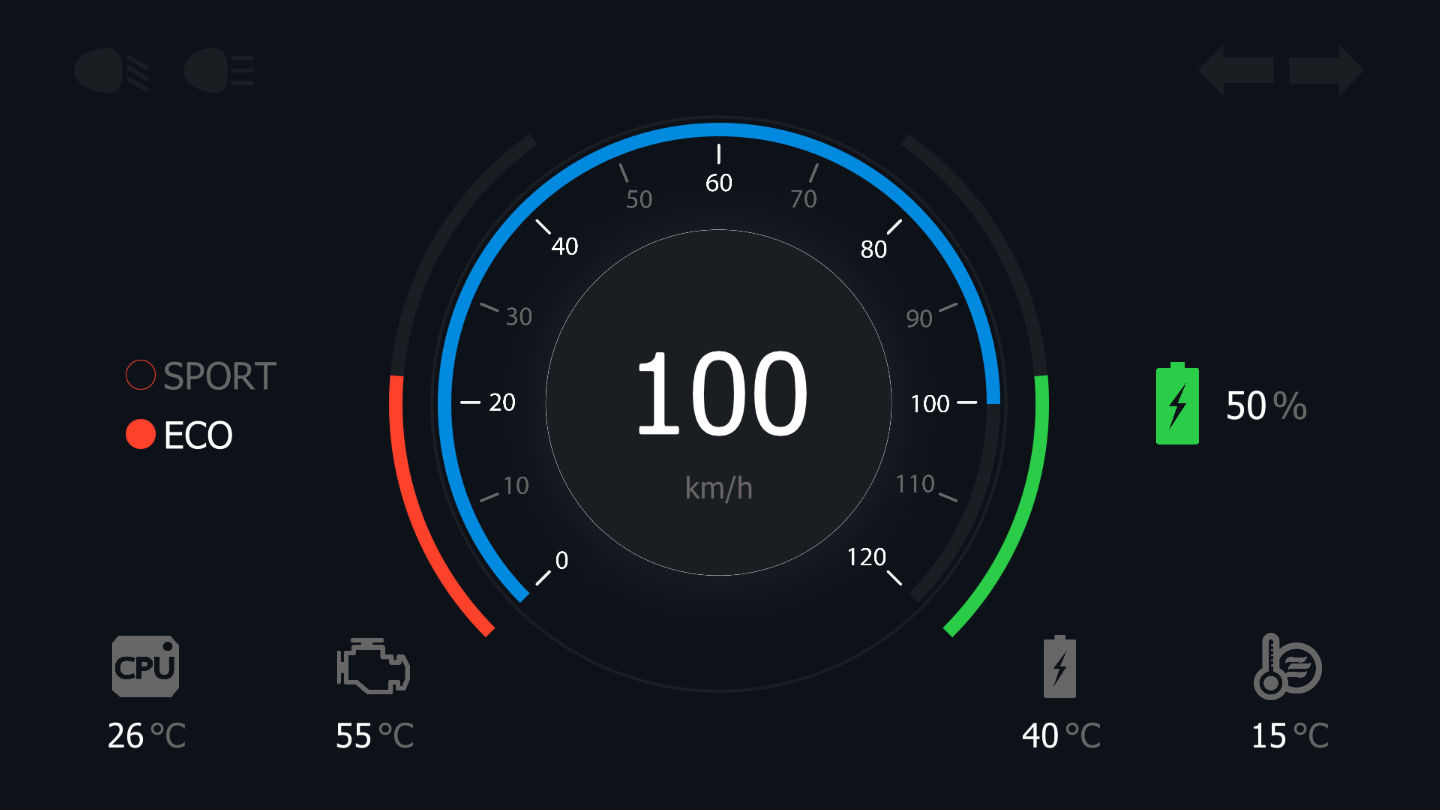
\includegraphics[scale=0.24]{figures/hcis/window_dashboard.png}
			\caption{GUI Fenster - Fahrdaten Diagnose}
			\label{fig:pageDiagnose}
	\end{center}
\end{figure}

\subsubsection{Errors}

\begin{figure}[H]
	\begin{center}
		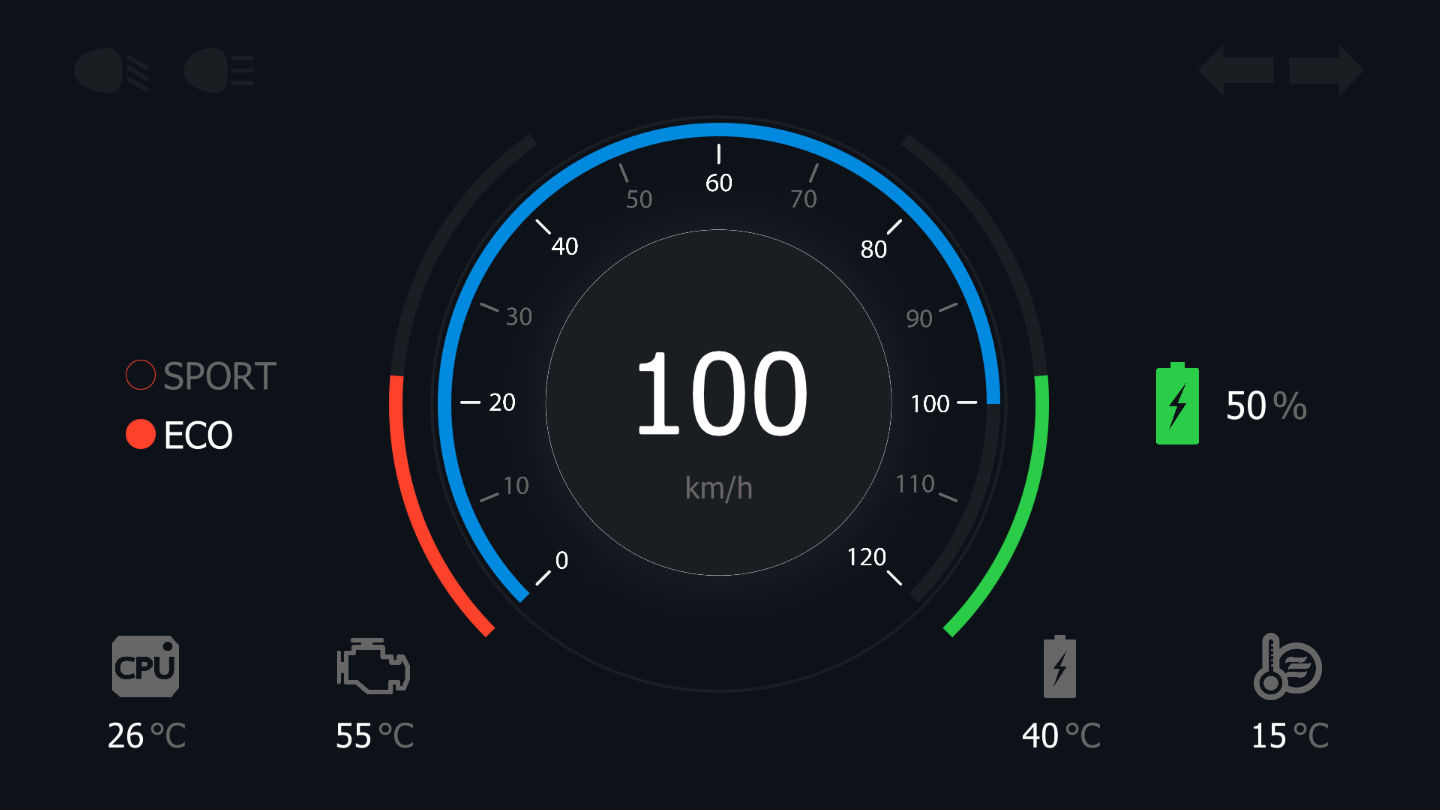
\includegraphics[scale=0.24]{figures/hcis/window_dashboard.png}
			\caption{GUI Fenster - Error List}
			\label{fig:pageError}
	\end{center}
\end{figure}

\newpage

\subsection{Realisierung der Benutzeroberfäche}

\subsubsection{QML}
QML ist eine deklarative Sprache, mit der Benutzeroberflächen anhand ihrer visuellen Komponenten und ihrer Interaktion und Beziehung zueinander beschrieben werden können. Es ist eine gut lesbare Sprache, die entwickelt wurde, um die dynamische Verbindung von Komponenten zu ermöglichen und die die einfache Wiederverwendung und Anpassung von Komponenten innerhalb einer Benutzeroberfläche erlaubt. Es bietet  Syntax mit Unterstützung für JavaScript-Ausdrücke in Kombination mit dynamischen Eigenschaftsverbindungen.

\subsubsection{Qt-Quick}
Das Qt-Quick-Modul ist die Standardbibliothek zum schreiben von QML-Anwendungen. Während das QML-Modul die Engine und die Sprachinfrastruktur bereitstellt, bietet das Qt Quick-Modul alle grundlegenden Typen, die zum Erstellen von Benutzeroberflächen mit QML erforderlich sind. Es bietet eine visuelle Zeichenfläche und Typen zum Erstellen und Animieren visueller Komponenten, zum Empfangen von Benutzereingaben, zum Erstellen von Datenmodellen und Ansichten sowie zum verzögerten Objektinstanziieren. Es können problemlos flüssige, animierte Benutzeroberflächen in QML erstellt werden. Diese Benutzeroberflächen können mit beliebigen back end Bibliotheken verbunden werden.

\subsubsection{Slots und Signals} \label{sec:slots}
Slots und Signals werden in Qml zur ereignisgesteuerte Kommunikation zwischen front end und back end verwendet. In der folgenden Illustration wird diese anhang eines einfachen Beispiels erklärt.

\begin{figure}[H]
\begin{center}
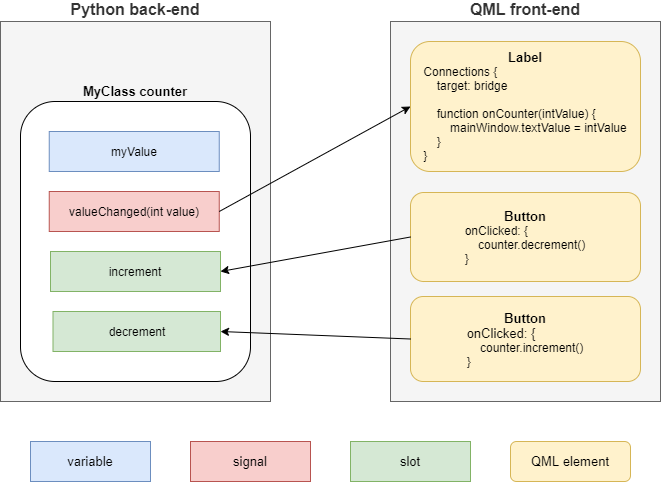
\includegraphics[scale=0.4]{figures/hcis/signals_slots.png}
\caption{Slots und Signals Konzept}
\end{center}
\end{figure}

\textbf{Signale}\\ \medskip
Diese können als Mitteilungen angesehen werden, welche über das Aufrufen der signal.emit funktion vom back-end an das Front-End gesendet wird. Im Front-End wird wiederum eine eigens definierte Funktion benötigt um dem Wert einem Property eines QML Elements zuzuweisen.
\medskip

\textbf{Slots}\\ \medskip
Slots sind Call-Back Funktionen, welche im Back-End definiert werden und sind über die Bridge Class mit dem Front-End verknüpft. Dadurch können diese Funktionen im Front-End aufgerufen und mit Signalen verbunden werden. Sie stellen daher die wichtigste Verbindung zwischen dem Programm und der Benutzeroberfläche dar.

\newpage
	
\subsubsection{Bridge}

\newpage

%% Kommunikation %%%%%%%%%%%%%%%%%%%%%%%%%%%%%%%%%%%%%%%%%%%%

\section{Kommunikation}
Um Daten zwischen den mehreren Steuereinheiten des Motorrades zu versenden, muss eine echtzeit Kommunikation über ein Bussystem gewährleistet werden. Die Entscheindung ist auf das Controller Area Network Bussystem (CAN-Bus) gefallen. Auschlaggebend für diese Entscheidung war der Curtis Motorcontroller, dieser verfügt über eine serielle Schnittstelle (RS-232) sowie ein CAN-System. Für unserer Anwendung bietet das CAN-System eine größere Ausbaufähigkeit sowie größere Übertragungsraten, weshalb wir uns letztendlich auch dafür entschieden haben.
\subsection{Hardware}
\subsubsection{CAN-Modul}
Da der Raspberry Pi selbst nicht über ein CAN-System verfügt, erfolgt der Anschluss an die Busleitung über ein externes CAN-Modul, welches über das Serial Peripheral Interface (SPI) mit dem Raspberry Pi kommuniziert, welches wie folgt angeschlossen werden muss: 
\begin{figure}[H]
	\begin{center}
		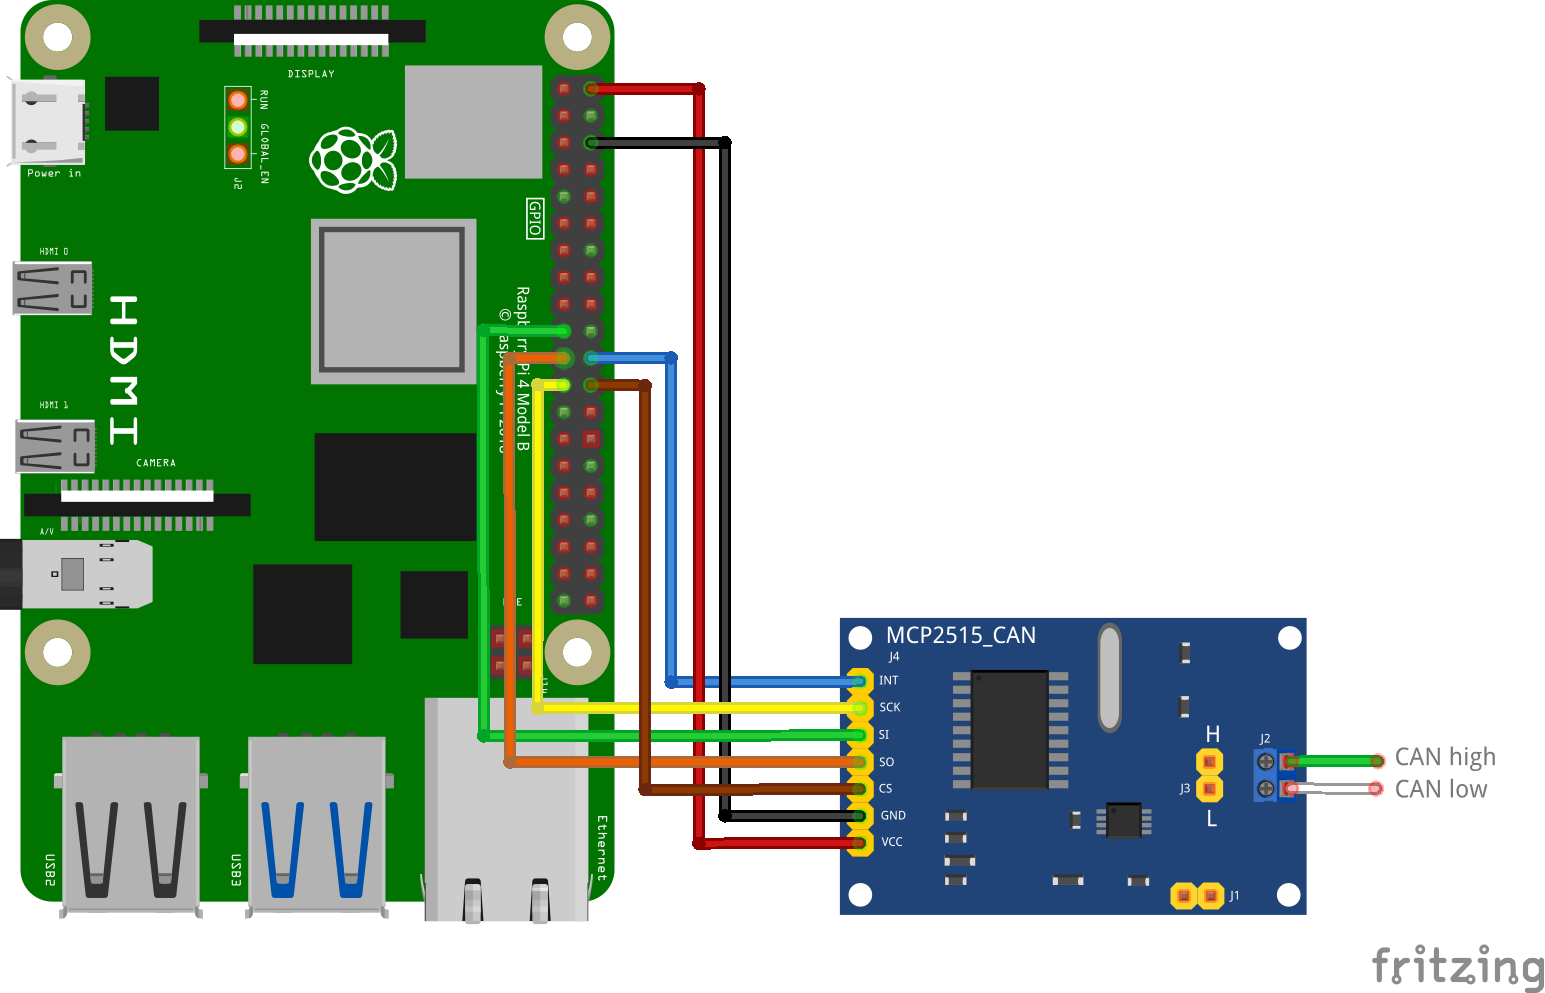
\includegraphics[scale=0.9]{figures/hcis/can_module.png}
		\caption{Anschlussplan CAN-Modul}
	\end{center}
\end{figure}

Die Kommunikation wird über zwei Komponenten ermöclicht. Einen MCP2562 Transceiver, welcher für die Verabeitung der Nachrichten zuständig ist und ein MCP2515 CAN Interface, welches die Daten zwischenspeichert und sich um das Versenden der Nachrichten kümmert. Gemeinsam mit dem Mircocomputer ergibt dies nun eine CAN Node, welche fähig ist Nachrichten zu versenden und zu empfangen.

\subsubsection{Netzwerkstruktur}

Ein CAN-Netzwerk wird standartmäßig als Linienstuktur oder Sternsturktur aufgebaut. Wir haben uns bewusst für ein Liniensystem entschieden, da Sternsysteme nur in bestimmten Anwendungen gebrauch finden und noch dazu markante Nachteile besitzt.\\ Es müsste zum Beispiel eine Zentrale Steuereinheit den Nachrichtenverkehr steuern, ebenso gibt uns die niedrige Anzahl an Teilnehmern im Netzwerk nicht einmal die Möglichkeit ein anderes System zu verwenden. Erst wenn wir in Zukunft das CAN-Netwerk um Sensoren und Aktoren erweitern würden, müsste weitere Zeit in die Planung des Netzwerks investiert werden. 

\newpage

\subsection{Listener}
\subsubsection{Receive Data}

\newpage

%% Fahrdatenspeicher %%%%%%%%%%%%%%%%%%%%%%%%%%%%%%%%%%%%%%%%

\section{Fahrdatenspeicher}
\subsection{Datenbankstruktur}
\subsubsection{Login System}
\subsubsection{Motor Daten}
\subsubsection{Akku Daten}
\subsection{Handler}
\subsubsection{SELECT Befehl}
\subsubsection{INSERT Befehl}

\newpage